\documentclass[letterpaper,10pt]{article}

\usepackage{titling}
\usepackage{listings}
\usepackage{url}
\usepackage{setspace}
\usepackage{subfig}
\usepackage{sectsty}
\usepackage{pdfpages}
\usepackage{colortbl}
\usepackage{multirow}
\usepackage{relsize}
\usepackage{amsmath}
\usepackage{fancyvrb}
\usepackage{amsmath,amssymb,amsthm,graphicx,xspace}
\usepackage[titlenotnumbered,noend,noline]{algorithm2e}
\usepackage[compact]{titlesec}
\usepackage{paratype} 
\usepackage[T1]{fontenc}
\usepackage{tikz}
\usetikzlibrary{arrows,automata,shapes,trees,matrix,chains,scopes,positioning,calc}
\tikzstyle{block} = [rectangle, draw, fill=blue!20, 
    text width=2.5em, text centered, rounded corners, minimum height=2em]
\tikzstyle{bw} = [rectangle, draw, fill=blue!20, 
    text width=4em, text centered, rounded corners, minimum height=2em]

\definecolor{namerow}{cmyk}{.40,.40,.40,.40}
\definecolor{namecol}{cmyk}{.40,.40,.40,.40}

\let\LaTeXtitle\title
\renewcommand{\title}[1]{\LaTeXtitle{\textsf{#1}}}


\newcommand{\handout}[5]{
  \noindent
  \begin{center}
  \framebox{
    \vbox{
      \hbox to 5.78in { {\bf ECE254: Operating Systems and Systems Programming } \hfill #2 }
      \vspace{4mm}
      \hbox to 5.78in { {\Large \hfill #4  \hfill} }
      \vspace{2mm}
      \hbox to 5.78in { {\em #3 \hfill} }
    }
  }
  \end{center}
  \vspace*{4mm}
}

\newcommand{\lecture}[3]{\handout{#1}{#2}{#3}{Lecture #1}}
\newcommand{\tuple}[1]{\ensuremath{\left\langle #1 \right\rangle}\xspace}

\addtolength{\oddsidemargin}{-1.000in}
\addtolength{\evensidemargin}{-0.500in}
\addtolength{\textwidth}{2.0in}
\addtolength{\topmargin}{-1.000in}
\addtolength{\textheight}{1.75in}
\addtolength{\parskip}{\baselineskip}
\setlength{\parindent}{0in}
\renewcommand{\baselinestretch}{1.5}
\newcommand{\term}{Spring 2015}

\singlespace


\begin{document}

\lecture{ 2 --- Review of Computer Architecture }{\term}{Jeff Zarnett}

\section*{Computer Organization}
Although a regular program like a word processor need not be concerned with the underlying hardware of the computer, this abstraction does not come for free: the operating system must be aware of these details and manage them for everyone. What is a program, anyway? You will know from your programming experience that a program is just a sequence of instructions and some data. Thus, to execute a program, we will need a few things:

\begin{enumerate}
	\item \textbf{Main Memory} -- a place where the instructions and data are stored;
	\item \textbf{System Bus} -- a way for instructions and data to travel between memory and the processor; and
	\item \textbf{Processor} -- that critical element of the system that actually executes the instructions.
\end{enumerate}

Of course, this is the minimal set; the modern personal computer tends to look more like this:

\begin{center}
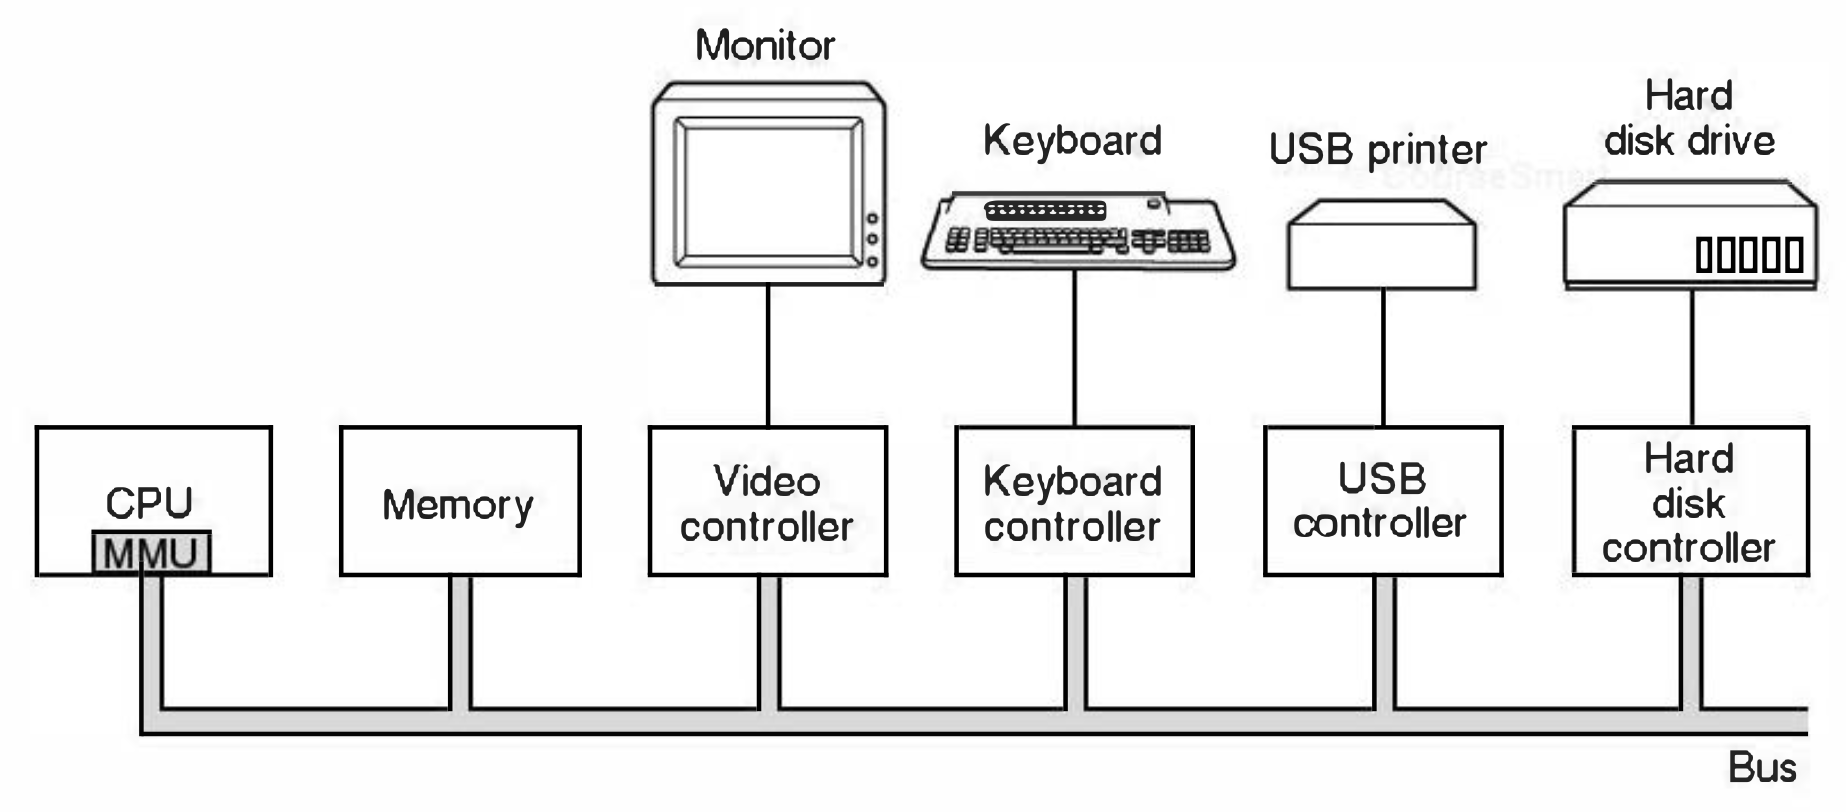
\includegraphics[width=0.75\textwidth]{images/modernpc.png}\\
Some components of a simple personal computer~\cite{mos}.
\end{center}

In the above diagram we have a fourth element: \textbf{Input/Output} (I/O). While not strictly necessary to run a program, a computer with no input or output devices is of, at best, limited usefulness.

\subsection*{Main Memory}
Ideally, memory would be fast enough that the processor never has to wait for memory, large enough to hold all the data of the system, and inexpensive. Readers familiar with reality will recognize this as the \textit{Iron Triangle}: ``fast, good, cheap; pick two.'' The good news is that we do not have to make only one choice. We can have different levels of memory at different sizes, speed, and cost. You are presumably already familiar with this because a typical laptop has both RAM (Random Access Memory) and a hard drive (or solid state drive) and they are not only different sizes, but follow independent pricing schemes. Moving from 4 GB of RAM to 8 GB of RAM might cost the same as a change from a 1 TB hard drive to a 2 TB hard drive. So what we end up with is a hierarchy of memory. Let us compare the various levels I might have in my laptop from 2013:

\begin{center}
	\begin{tabular}{l|l|l}
	\textbf{Memory Level} & \textbf{Access Time} & \textbf{Total Capacity} \\ \hline
	Register & 1 ns & < 1 KB \\
	Cache & 2 ns & 6 MB \\
	Main Memory (RAM) & 10 ns & 16 GB \\
	Magnetic Hard Disk & 10 ms & 500 GB \\
	\end{tabular}
\end{center}

Notably, the cache (pronounced like ``cash'') is very often broken down into different levels like L1 (Level 1), L2, L3. In any case, the trend is clear: fast memory is expensive and as we get further away from the CPU memory access gets slower, but it gets less expensive so we can have more of it. 

The difference in access time is often quite dramatic. An analogy to put it in perspective: imagine I am the CPU and a particular book is the piece of data needed. If the data is in the cache, it is as if the book is on a bookshelf in my office. Thus, I can retrieve the book very quickly. If the data for the CPU on a magnetic hard disk, it is as if I would have to get the book from Library and Archives Canada in Ottawa (about 550 km away, according to Google Maps). And I would have to walk. Of course, the analogy is slightly tortured because the CPU doesn't go get the data; instead it must wait for it to arrive. If I ordered a book from Library and Archives Canada and someone had to walk it over, I would spend a lot of time waiting. What might I do in the meantime...?

Management of memory and caching will be a major topic to be examined later on.

\subsection*{System Bus(es)}
\begin{quote}
	\textit{The bits on the bus go up and down, up and down, up and down...}
\end{quote}

As you can imagine, with every sort of communication using the same bus, contention for this resource is a major limiting factor in the operation of the computer. It turns out, the diagram shown earlier with the single bus is a simplification (though the original IBM PC did work like that). A modern system has numerous buses that work at different speeds and towards different functions. The study of buses and their functions and problems are not something we will focus on, but it deserves mention as a key part of the hardware.

\subsection*{The Processor}

The Processor (or \textit{CPU}, central processing unit) is the brain of the computer. It fetches instructions from memory, via the bus, decodes the instruction, then executes it. This fetch-decode-execute cycle will be repeated until the program finishes (... if the program finishes). The different steps may be executed in parallel: while one instruction is being executed, the next is being decoded, and the one after that is being fetched. We call this a \textit{pipeline}, and the length and complexity of the pipeline is something we will not examine here, but is an interesting subject all its own. A processor's largest unit on which it operates is called a \textit{word}. A 32-bit processor has a word size of 32 bits and a 64-bit processor has a word size of 64 bits.

CPU instructions are, obviously, specific to the processor. If you have any experience in writing assembly code, you have probably used some books that tell you all the instructions that can be issued and what operands, if any, those instructions take. In some CPU architectures, some operations are available only in ``supervisor mode'' and not in ``user mode''. An instruction that disables interrupts is an example of an instruction that would be available only in supervisor mode. Attempting to run it in user mode will be an error.

In addition to the hardware to decode and execute the different instructions, the CPU has some storage locations called \textit{registers}. They may store data or instructions (they are both, after all, just a bunch of bits). Registers are a key concept in CPUs and management of those registers is partly the responsibility of the operating system. Registers are used to hold key variables and temporary results. Registers are often, but not always, word-sized. Let us examine some of the critical registers in processors.

\paragraph{Program Counter.} A program is a sequence of instructions, and as you can imagine, to execute one correctly, we need to keep track of what instruction is next. After the instruction at that address is fetched, the program counter is incremented. That points it to the next instruction, or, at least, a guess at the next instruction. As you know, programs often have conditional instructions and loops, so the the program counter may be updated to hold a different address than simply the ``next''.

\paragraph{Status Register.} The status register (sometimes called ``program status word'') is used as an array of bits to indicate various flags or properties, indicating the state of the processor. We can divide flags into two categories: arithmetic and non-arithmetic. The arithmetic flags are used to indicate mathematical outcomes, such as an overflow (e.g., the result of an operation was too large to fit in a register), or division by zero error. The non-arithmetic flags may be used to note that the CPU is running in supervisor mode rather than user mode, or that an assembly instruction was invalid. Complex CPUs may have more than one status register. 

\paragraph{Instruction Register.} The instruction most recently fetched will then be stored in the instruction register. Nothing complex or exciting here.

\paragraph{Stack Pointer.} The CPU may have a specific register to indicate the location in memory that is at the top of the stack. You will remember that memory in an executing program is divided, logically, into two separate categories: the stack and the heap. It is convenient to maintain a handy reference to the top of the stack in memory.

\paragraph{General Purpose Registers.} General purpose registers may store data as well as addresses. A typical arithmetic instruction like addition requires data to be loaded into these general purpose registers and stores the result in those general purpose registers. Usually the compiler determines how they are used, but in C you can exercise some measure of control using the \texttt{register} and \texttt{volatile} keywords.

This is not an exhaustive list, however. There may be others in a system like the memory address register, memory buffer register, I/O address register...


\section*{Program Execution}

As mentioned earlier, a program to execute is just a set of instructions, telling the CPU what to do. The processor retrieves the next instruction from the instruction register and will decode it (and thus figure out what to do). According to~\cite{osi} we can categorize these actions into one of the following categories:

\begin{enumerate}
	\item \textbf{Processor-Memory:} Transfer data from a processor to memory or vice versa (e.g, read an int from memory).
	\item \textbf{Processor-I/O:} Transfer data to or from an I/O device (e.g., make the speaker beep).
	\item \textbf{Data Processing:} Perform some arithmetic or logical operation on data (e.g., add two numbers).
	\item \textbf{Control:} Alter the sequence of execution (e.g., go back to the start of the loop).
\end{enumerate}


\subsection*{Interrupts}

As discussed earlier, if I have ordered a book from Library and Archives Canada it will take quite a long time for someone to walk the book to my office in Waterloo, and I would spend a lot of time waiting. So in the meantime, it seems logical that I should do something else. There are two options for dealing with this situation. One is polling: that I can check periodically if the book has arrived. This approach is fairly wasteful (how often do I check? How much time will I spend checking?). The other solution is that I can receive a notification when the poor fellow who has walked the 550 km to my office has arrived. If he knocks on my office door, it will cause me to suspend what I am doing and collect the book. Or, to put it in one word: interrupts.

In that analogy I played the part of the CPU, and was interrupted and had to deal with that interruption. We have the same in computer systems. When an interrupt happens, the normal sequencing of the processor does not continue. Interrupts are, according to~\cite{osi}, also something we can categorize into four buckets, based on where they are generated from:

\begin{enumerate}
	\item \textbf{Program:} Something happens in the program (e.g., a division by zero).
	\item \textbf{Timer:} A configured timer within the processor's time expires (e.g., to update the system clock).
	\item \textbf{Input/Output} An I/O controller signals (un)successful completion of an operation (e.g., read from disk).
	\item \textbf{Hardware Failure} Something happens in hardware (e.g., power failure).
\end{enumerate}

Interrupts are primarily a way to improve processor utilization (i.e., the fraction of the time the CPU is doing useful work). CPU time is valuable and the CPU can and should do something else while it is awaiting the results of some other operation. Thus, the CPU might issue a read from memory instruction, work on something else, and then be interrupted when the data has arrived from memory.

When an interrupt takes place, the processor might choose to ignore it, but this is rare. Interruptions usually contain important information. Almost always, we will want to \textit{handle} (deal with) the interrupt in some way.

Consider an analogy with which you are surely familiar: a professor is at the front of the lecture hall droning on about some subject. A student raises her hand to ask a question. The professor can ignore this, but that is generally a bad idea. The professor should pause what he is doing (pause execution), remembering where he was (save state), take the question and answer it (handle the interrupt), and then resume from where he left off (restore the saved state and continue execution).

The operating system is responsible for storing the state of the program being interrupted, handling the interrupt, and then restoring the state of the program that was interrupted.

Sometimes the CPU is in the middle of something where an interruption would be bad. Thus, interrupts can be disabled. This is like the professor saying that all questions should be saved until the end of the lecture. Once interrupts are enabled again, the interruptions can be handled. So all the questions that students have saved can be answered. Interrupts tend to have a priority, so if multiple interrupts are pending, the highest priority one will be dealt with first.

There can also be multiple interrupts happening in a short period of time: suppose interrupt 1 occurs and then interrupt 2 occurs while interrupt 1 is still being handled. Often, but not always, interrupt handlers themselves disable interrupts so a subsequent interrupt will be handled after the current one is dealt with. Or, interrupt 2 may itself interrupt the first. Consider the diagrams below:

\begin{center}
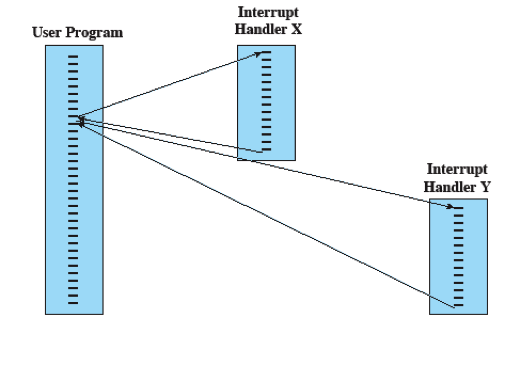
\includegraphics[width=0.45\textwidth]{images/interrupts-sequential.png}
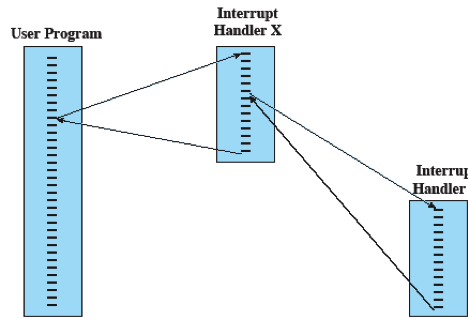
\includegraphics[width=0.45\textwidth]{images/interrupts-nested.png}\\
Left: Sequential interrupt handling. Right: Nested interrupt handling.~\cite{osi}
\end{center}

A combination of these different techniques may be used. A low priority interrupt handler may be suspended to deal with a high priority interrupt. Suppose while the high priority interrupt is being handled, a medium priority interrupt occurs. The high priority interrupt handler will be allowed to complete its work before the medium priority interrupt is dealt with.


\paragraph{Storing and Restoring State.} We mentioned already that the operating system is responsible for storing the state of the program (or interrupt handler) being interrupted when an interrupt !`occurs. To do so, the state of the CPU is what must be stored. The values of the various registers (e.g., program counter, instruction register, etc.) are stored by pushing them onto the stack. When the interrupt is finished, those values are popped off the stack and loaded into the registers again. After that, program execution continues (almost) as if the interruption never took place.

\paragraph{Multiprogramming.} Thus far we have assumed that there is a program running and that same program is the one that resumes at the end of the interrupt handling. This is, however, not always the case. Given that we have stored the state of the interrupted program, we can resume it any time we like, and run a different program now instead. But which program should we run next? We will examine the subject when we talk about scheduling.

\subsection*{I/O Communication}
That fourth major element of the modern computer system, I/O, is something we have thus far not examined. Now we will consider three strategies for I/O operations, each of which we can examine briefly. In the examples we will assume the operation to be completed is a read, but writing is the same, just in the opposite direction.

\paragraph{Programmed I/O.}  This strategy is really just the name for polling. The processor issues an I/O command and is responsible for checking when the I/O operation is complete. This usually requires checking the I/O device's status register or memory location. The I/O device updates this when it has financed the operation. Polling is, however, an inefficient way to get things done. The CPU is either waiting around doing nothing or checking the status register. Once the status has been checked and indicates finished, the CPU can copy the data into memory.

\paragraph{Interrupt-Driven I/O.} Interrupts are a much more efficient way to get things done. The CPU issues the read or write and eventually, when the operation is completed, the I/O module issues an interrupt to indicate it is finished. At that point the CPU will copy the data into memory.

In both the interrupt and programmed I/O strategy, the CPU is involved twice: it initiates the read (or write) and then collects the result and does something with it. The read has three parties: the device, the CPU, and memory. What if we could eliminate the middleman (the CPU) from this equation?

\paragraph{Direct Memory Access (DMA).} The most efficient way to handle a large block of data is with DMA. The advantage to DMA is that the CPU is involved in setting up the operation but does not have to manage things. It introduces the I/O device and memory to one another and says ``you figure it out''. The CPU will do some set up, indicating:

\begin{enumerate}
	\item The operation to perform (read or write)
	\item The source
	\item The destination
	\item How much data is to be transferred
\end{enumerate}

This data is sent to the DMA module (a delegate). After that, the CPU can go on to do other work and the I/O device will interact directly with memory. Hence, the name, Direct Memory Access. Note that the CPU may have to contend with the DMA operation for the bus, but even if this is the case, it is more efficient to use DMA than either interrupt or programmed I/O ~\cite{osi}.

\bibliographystyle{alpha}
\bibliography{254}


\end{document}